
\chapter{ABCD rules, and Dermoscopic Structures}

\section{Introduction}
This chapter is a discussion of the most popular ABCD (Asymmetry, Border, Colour, and Dermoscopic Features) algorithms including their implementation, and updating the algorithms. They are compared using the PH2 dataset and updated relating to their accuracy. Surprisingly, many of the ABCD rules techniques were originally tested for whether they effectively find melanoma and not individual features. So, this will be the first time some of these techniques have been tested and documented.

\section{ABCD Rules Data Extraction Techniques}
The automatic detection of ABCD rules for the detection of ABCD rules has warranted extensive research and development\cite{Ali2020}. The ABCD rules stand for Asymmetry, Border irregularity, Colour variegation, and Diameter greater than 6mm, and have been fundamental framework for the clinical diagnosis of melanoma. Sometimes Diameter is changed for Dermoscopic structures because measruing the size of the lesion is not always possible when capturing an image. Furthermore, demroscopic structures provides further insight into diagnosing melanoma\cite{}. Another useful change made to the ABCD rules is E for evolution, showing that it changes overtime, datasets however do not support this. Although the diagnostic procedures ABCD rules is frequently used in the medical environment it has limitations in detection of small melanomas and those with resular shape and homoheneous colour\cite{Argenziano2006}. As a result, automatic classification algorithms for ABCD rules has become more prevelant\cite{Kasmi2016}.

The benefits of implementing a CAD system for the automatic detection of ABCD rules is the classification of exisiting diagnostic procedure in which clinicians are already aware of how it fundementally works. Another benefit is the automatic labelling of data, where it would take considerable time to input this diagnostic data into a server for further analysis, where the automatic system could generate results and the clinician only needs to check whether these results are correct. Other benefits include improving objectivity of results, where normally ABCD rules is considered subjective, meaning it can be utilised in a variety of ways. This ultimietly makes comparisons very difficult between lesions, but automatic detection can improve the objectivity, making hospital wide comparisons easier. Check out the previous chapter discussing the PH2 dataset and the data subjectivity on page\pageref*{ph2-image-assessment}.

\subsection{Asymmetry Techniques}
Asymmetry analysis is a fundamental component in the early detection of melanoma because it often exhibits asymmetric shapes\cite{Ali2020a}. Meaning that the shape, colour and, texture match asymmetrically more often in benign lesions. For example, as melanoma grows the central area begins to waste away leaving a hollow area covered by thin skin, showing dermoscopic features. As it grows the edges become more irregular producing an uneven shape often relating to irregular borders and asymmetrical shapes. Diagnostic procedures have been developed to detect these unique characteristics.

\begin{figure}
    \centering
    %\includegraphics[scale=1.2]{images/asymmetry/.png}
    \caption{} 
\end{figure}\label{asy-examples}

\begin{figure}
    \centering
    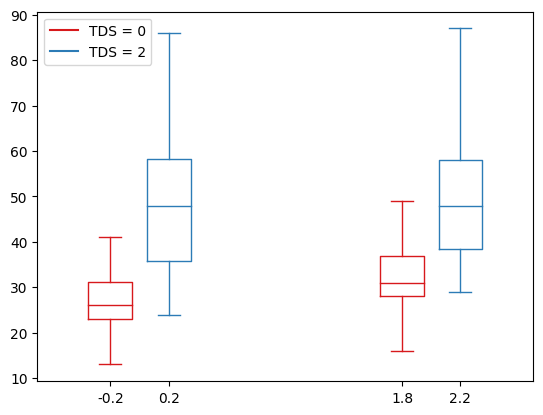
\includegraphics[scale=1.2]{images/asymmetry/asy-changes.png}
    \caption{} 
\end{figure}\label{asy-changes}

Figure\ref{asy-changes} demonstrates the difference between the updated asymmetry algorithm using super pixels compared with the original

the asymmetry algorithm using super pixels decreases the median and range, compared with the original method where the pixels are closer together

%Tables showing the accuracy of all three of the techniques essentially showing that segnet is obviously better.


\section{A Novel Asymmetry detection technique using Bi-Fold, 3D Euclidean distance, and Superpixels}
This section describes a novel machine-learning technique for the automatic detection of melanoma

\subsection{Image Transformation}
Transforming the skin lesion image is important to prevent scale variance in the algorithms. For example some of the images have a smaller skin lesion in upper corners and others take up the entire image size. For adequate comparisons the images must be transformed to match sizes. THis ensures the images are being compared fairly.

To transform the image it is converted to gray scale and a threshold is applied finding all non-zero pixels. This is followed by a bounding rectangle around the area being assigned. After this the assigned area from the original image is cropped.

\begin{figure}
    \centering
    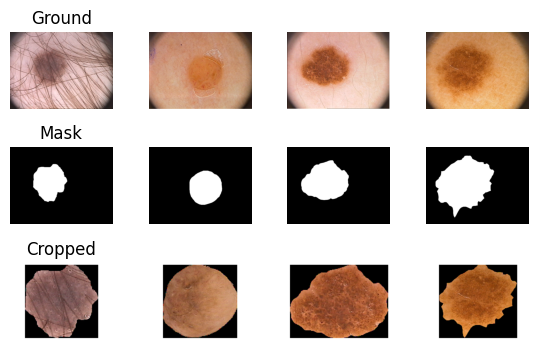
\includegraphics[scale=1.2]{images/asymmetry/asy-cropped.png}
    \caption{This figure shows some images from the PH2 dataset after being masked, cropped, and rotated using bi-fold.} 
\end{figure}\label{asy-cropped}

%Diagram showing the image before and after transformation
The first line in figure \ref{asy-cropped} shows the skin lesion image, the second shows the segmentation mask, and the third shows the images after being cropped and rotated using bi-fold.

\subsection{Bi-fold}
Bi-fold is a diagnostic procedure designed to support the recognition of melanoma by drawing a line down the middle of the skin lesion and comparing the two halves to confirm whether the sides match (considering the difference in shape, colour, and texture). Using this horizontally and vertically calculates whether the skin lesion is possibly malignant with a score between 0 and 2. Calculating with Total Dermoscopy Score (TDS) alongside the other ABCD rules including asymmetry, border, colour, and diameter calculates the likelihood of malignancy. Dermatologists frequently use bi-fold due to its simplicity, but it can be subjective to the original observer and time-consuming when managing large numbers of skin lesions. Therefore, automating techniques is beneficial to clinicians and can improve the objectivity of results.

To initiate the classification of skin lesions a technique called bi-fold is applied involving folding the skin lesion in half vertically and horizontally and a comparison of their respective dimensions. While the original technique was designed only to assess the lesions' shape, it's been utilized to account for colour and texture as well. The centre and orientation are determined by calculating its moments, where the centre is (m10 / m00, m01 / m00) and phi is 0.5tan (2m11)/ (m20 -m02).

%Add diagram demonstrating bi-fold of a skin lesion
\begin{figure}
    \centering
    %Make better images showing both vertical and horizontal rotation after analysis
    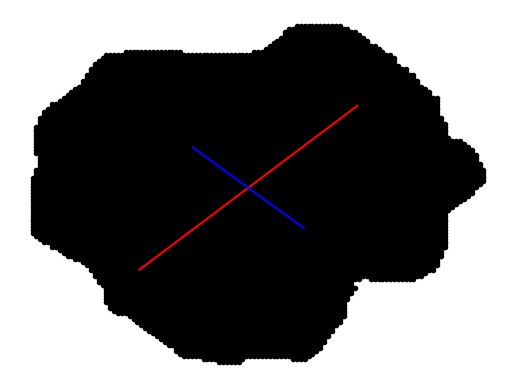
\includegraphics[scale=0.5]{images/asymmetry/bi-fold1.png}
    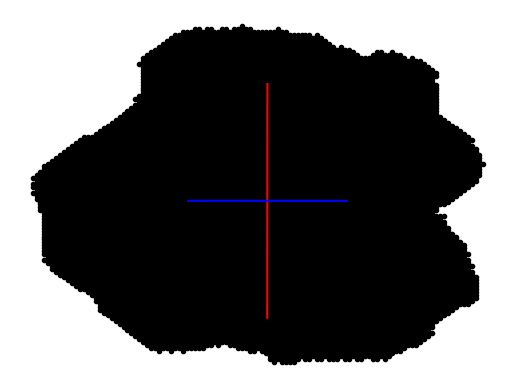
\includegraphics[scale=0.5]{images/asymmetry/bi-fold1-rotated.png}
    \caption{This diagram shows image IMD003 from the PH2 dataset after calculating Bi-fold, followed by rotating the image to match the rotation defined using moments of inertia.} 
\end{figure}\label{asy-bifold}

\subsection{Shape analysis}
Analysing the shape of the skin lesion 

\subsection{3D Euclidean Distance}
Next, the lesion is partitioned into a 20 by 20 grid centred on the mentioned centre point, and the average of each region is computed. This is followed by finding the matching region on the perpendicular area from the centre of the skin lesion and comparing the colour distance between the two. Distance is measured using the LAB colour space and a 2D Euclidean distance of A and B, removing L (luminosity) to eliminate light variation. Once compared, all compared regions are obtained, and they are plotted onto a graph. If over half of the values are above a threshold of 6, then the lesion is asymmetrical.

% Scrutinize the threshold method and show the graph that the data can't be split with only the threshold 
The diagram shown below in figure\ref{symmetrical} is a compilation of all the images within the PH2 dataset showing the threshold range after applying bi-fold, euclidean distance of colour, but before applying the threshold. As can be seen, a threshold of 6 covers all of the symmetrical values, but still roughly covers half of the asymmetrical values. This demonstrates that the technique produces many false positives when regarding asymmetrical values.
Essentially, the symmetrical skin lesion has a smaller area and the asymmetrical lesion has a larger area, but both remain in the same zone and therefore splitting the data only using a threshold holds poor results. Furthermore, there are a lot of fliers and the threshold does not adjust according to these values. See the graph below:

\begin{figure} 
    \centering
    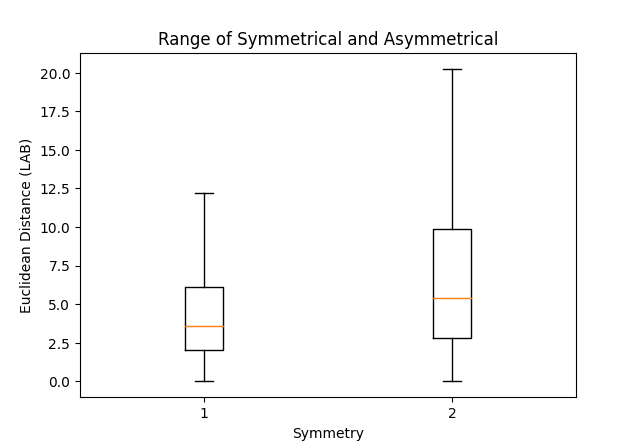
\includegraphics[scale=0.6]{images/symmetrical.png}
\caption{This diagram is a summary of the PH2 dataset after using bi-fold, a Euclidean distance of colour. The value on the right would be a threshold.}
\end{figure}\label{symmetrical}
    
To improve the accuracy of the algorithm some changes need to be made based on the previous statements. First will be superpixels and next is k-means.

\subsection{Superpixels using Simple Linear Iterative Clustering (SLIC)}
% Demonstrating the changes including superpixels and graphs, etc
Superpixel is an algorithm for grouping pixels into a grid format, but with flexible borders that can adjust to regions with similar features. Unlike the original technique averaging specific squares in a grid\cite{Kasmi2016}, they are segmented related to colour, texture, and other properties. The reason for using this technique is to increase boundary adherence and to group features that might otherwise be split into separate groups. This overall improves the accuracy of the algorithm.

This technique uses a simple linear iterative clustering (SLIC) algorithm and was first introduced by Achanta et al.\cite{Achanta2012}. The technique combines both k-means and graph-based segmentation. Firstly you define the desired number of superpixels as $k$ and the approximate size of each superpixel as $S$, which is usually $S = /square(N/k)$ and $N$ is the number of pixels in the image. Secondly, for the centre of each cluster, a search space is assigned to the cluster. For each group, you measure the spatial distance which is the Euclidean distance between each pixel and the cluster center. Each pixel is assigned to the cluster with the nearest centroid. The cluster centres are then recalculated by taking the mean colour and position of the pixels assigned to each cluster. Followed by new pixels being assigned to the centroid relating to Euclidean distance. This process is repeated depending on the number of iterations as $i$ are assigned. From this point, each pixel is assigned to a cluster.

The image in ... demonstrates the usual average and the new averages based on superpixels and the changes in values. Areas that are lighter in colour appear to have a lower value and darker appear darker.

Using the thresholding method for classification we can already see the accuracy has been improved with a threshold of ...

\section{Experimental Results}
The goal of this experiment is to improve the accuracy of the asymmetry bi-fold technique described by Ihab S. Zaqout et al.\cite{Zaqout2016}. Initially, the skin lesion is split into a 10 by 10 grid and converted into the LAB colourspace. Next, a line is drawn through the middle horizontally and vertically. Measuring the Euclidean distance from the centroid, locating the closest opposite patch of colour finds the parallel square. Subtracting the squares generates a score for each value, the closer to 0, the more similar the colour. These are then removed from the list to prevent them from being selected a second time. If half the results are over a specific threshold, it is considered asymmetrical in colour, otherwise considered symmetrical. The aim is to make a 10 by 10 grid, but instead of averaging squares, superpixels reduce data redundancy in the grid, allowing for a less complex algorithm and improving accuracy. The clustering method k-means partitions each pixel to its nearest most similar centroid relating to colour. Next, it generates a superpixel that represents the average colour of that area. The diagram\ref{SP} demonstrates different borders when changing the $C$ for compactness, where 100 generates a square grid similar to the original technique. The border becomes more flexible as the compactness value decreases.

\begin{figure} 
\centering
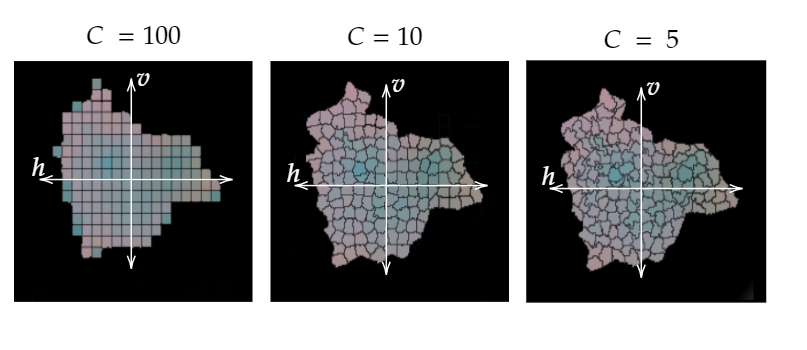
\includegraphics[scale=0.6]{images/superpixels.png}
\caption{This diagram shows the skin lesion split relating to superpixels instead of averaging squares.}
\end{figure}\label{SP}

Each parallel square on the vertical and horizontal axes measures similarity using a three-dimensional Euclidean distance in the LAB colour space. For example, the perceivable difference of colour to the human eye is a three-dimensional Euclidean distance of 6\cite{Myridis2014a}. Using similar logic, a value of 20 is the threshold, where any value over that amount is considered asymmetrical in colour. Next, each square is compared with its closest parallel square (relating to the line through the centre defined by the bi-fold) and removed from an array after being compared. The next improvement is to generate a unique threshold for the significance of each square. For example, using superpixels with the compactness of 10 has an accuracy of 61\% with the PH$^2$ dataset compared to the original 59.5\%. This approach demonstrates that a flexible border that considers features is more effective than averaging squares.

\begin{figure}
\centering
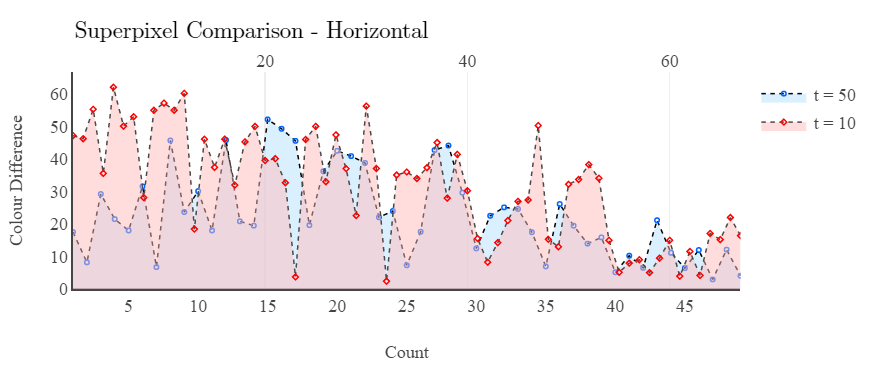
\includegraphics[scale=0.7]{images/superpixel2.png}
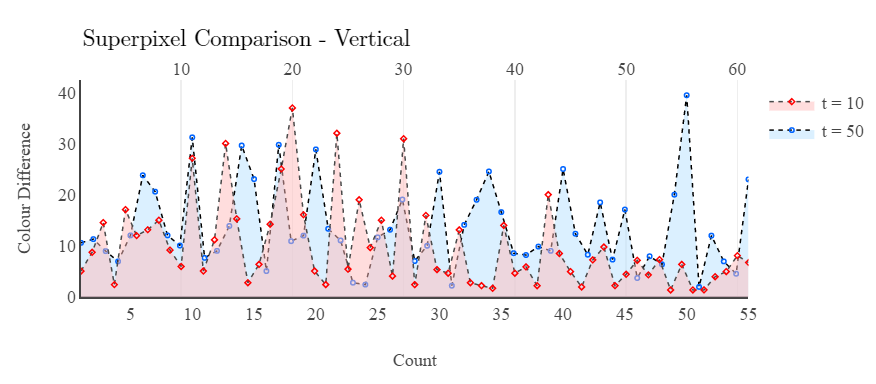
\includegraphics[scale=0.7]{images/superpixel1.png}
\caption{This diagram shows the difference between averaging squares and using superpixels, with the threshold of 10 implying curves and 50 being squares. The horizontal colour difference is improved, making it more likely to be seen asymmetrical. The vertical comparison is roughly the same, except for removing a false positive of 40.}
\end{figure}\label{asy3}

There is a correlation in colour differences between the inner and outer edges because melanoma typically expands outwards, creating an abnormal border. This information specifies that the statistical model accuracy could be improved by increasing the threshold for the outer edges and decreasing it for the inner.

\section{Border Detection Using Zernike Moments, 
Fractal Box-Counting, and Convexity}


\section{A Novel Colour Analysis Approach using Colour Ranges, and SVM}


\section{Dermoscopic structures}

\section{Results}


\section{Conclusion}

% Describe the asymmetry technique and the changes that have been made to it.

%The proposed method has many similarities to Kasmi and Mokrani\cite{Kasmi2016} colour comparison technique, except it is updated to improve accuracy using superpixels, and a Support Vector Machine (SVM).

%The original method uses moments of inertia

%without any flexibility splits areas of interest in half, making comparisons less adequate. Using superpixels allows for a softer border which improves colour separation and accuracy.

%Superpixels are k-means colour extraction techniques designed to separate areas of an image into their associated areas of colour by applying a soft border around the edge.